\documentclass[tikz,border=6pt]{standalone}
\usepackage[T1]{fontenc}
\usepackage{lmodern}
\renewcommand{\familydefault}{\sfdefault}
\usepackage{tikz}
\usetikzlibrary{arrows.meta,positioning,calc}

\definecolor{collect}{HTML}{2F5E8C}
\definecolor{collectbg}{HTML}{EEF4FA}
\definecolor{clean}{HTML}{2F7A66}
\definecolor{cleanbg}{HTML}{EEF8F5}
\definecolor{prep}{HTML}{B87523}
\definecolor{prepbg}{HTML}{FCF3E8}
\definecolor{analysis}{HTML}{7A4F9E}
\definecolor{analysisbg}{HTML}{F5EFFA}
\definecolor{ink}{HTML}{1D1D1F}
\definecolor{muted}{HTML}{5C6166}
\definecolor{linegray}{HTML}{A8AEB6}
\definecolor{softgray}{HTML}{F5F6F7}

\tikzset{
  >={Latex[length=2.8mm,width=2.0mm]},
  stage/.style={rounded corners=7pt, line width=1.1pt, minimum height=13.2cm, inner sep=0pt},
  stagehead/.style={rounded corners=7pt, minimum height=0.95cm, text=white, font=\bfseries\fontsize{12}{13}\selectfont, inner sep=0pt},
  modulebox/.style={rounded corners=5pt, line width=0.9pt, fill=white, align=left, inner sep=7pt},
  handoff/.style={rounded corners=5pt, line width=0.9pt, align=center, inner sep=6pt, font=\fontsize{8.0}{9.1}\selectfont},
  flow/.style={-{Latex[length=2.8mm,width=2.2mm]}, draw=linegray, line width=1.05pt},
  vflow/.style={-{Latex[length=2.4mm,width=1.8mm]}, draw=muted!80, line width=0.9pt},
  note/.style={rounded corners=4pt, draw=linegray!80, fill=softgray, line width=0.7pt, align=left, inner sep=5pt, font=\fontsize{8.2}{9.2}\selectfont},
}

\newcommand{\modtitle}[1]{{\bfseries\fontsize{9.7}{11}\selectfont #1}}
\newcommand{\modbody}[1]{{\fontsize{8.45}{9.6}\selectfont #1}}
\newcommand{\bul}{\textbullet\;}

\begin{document}
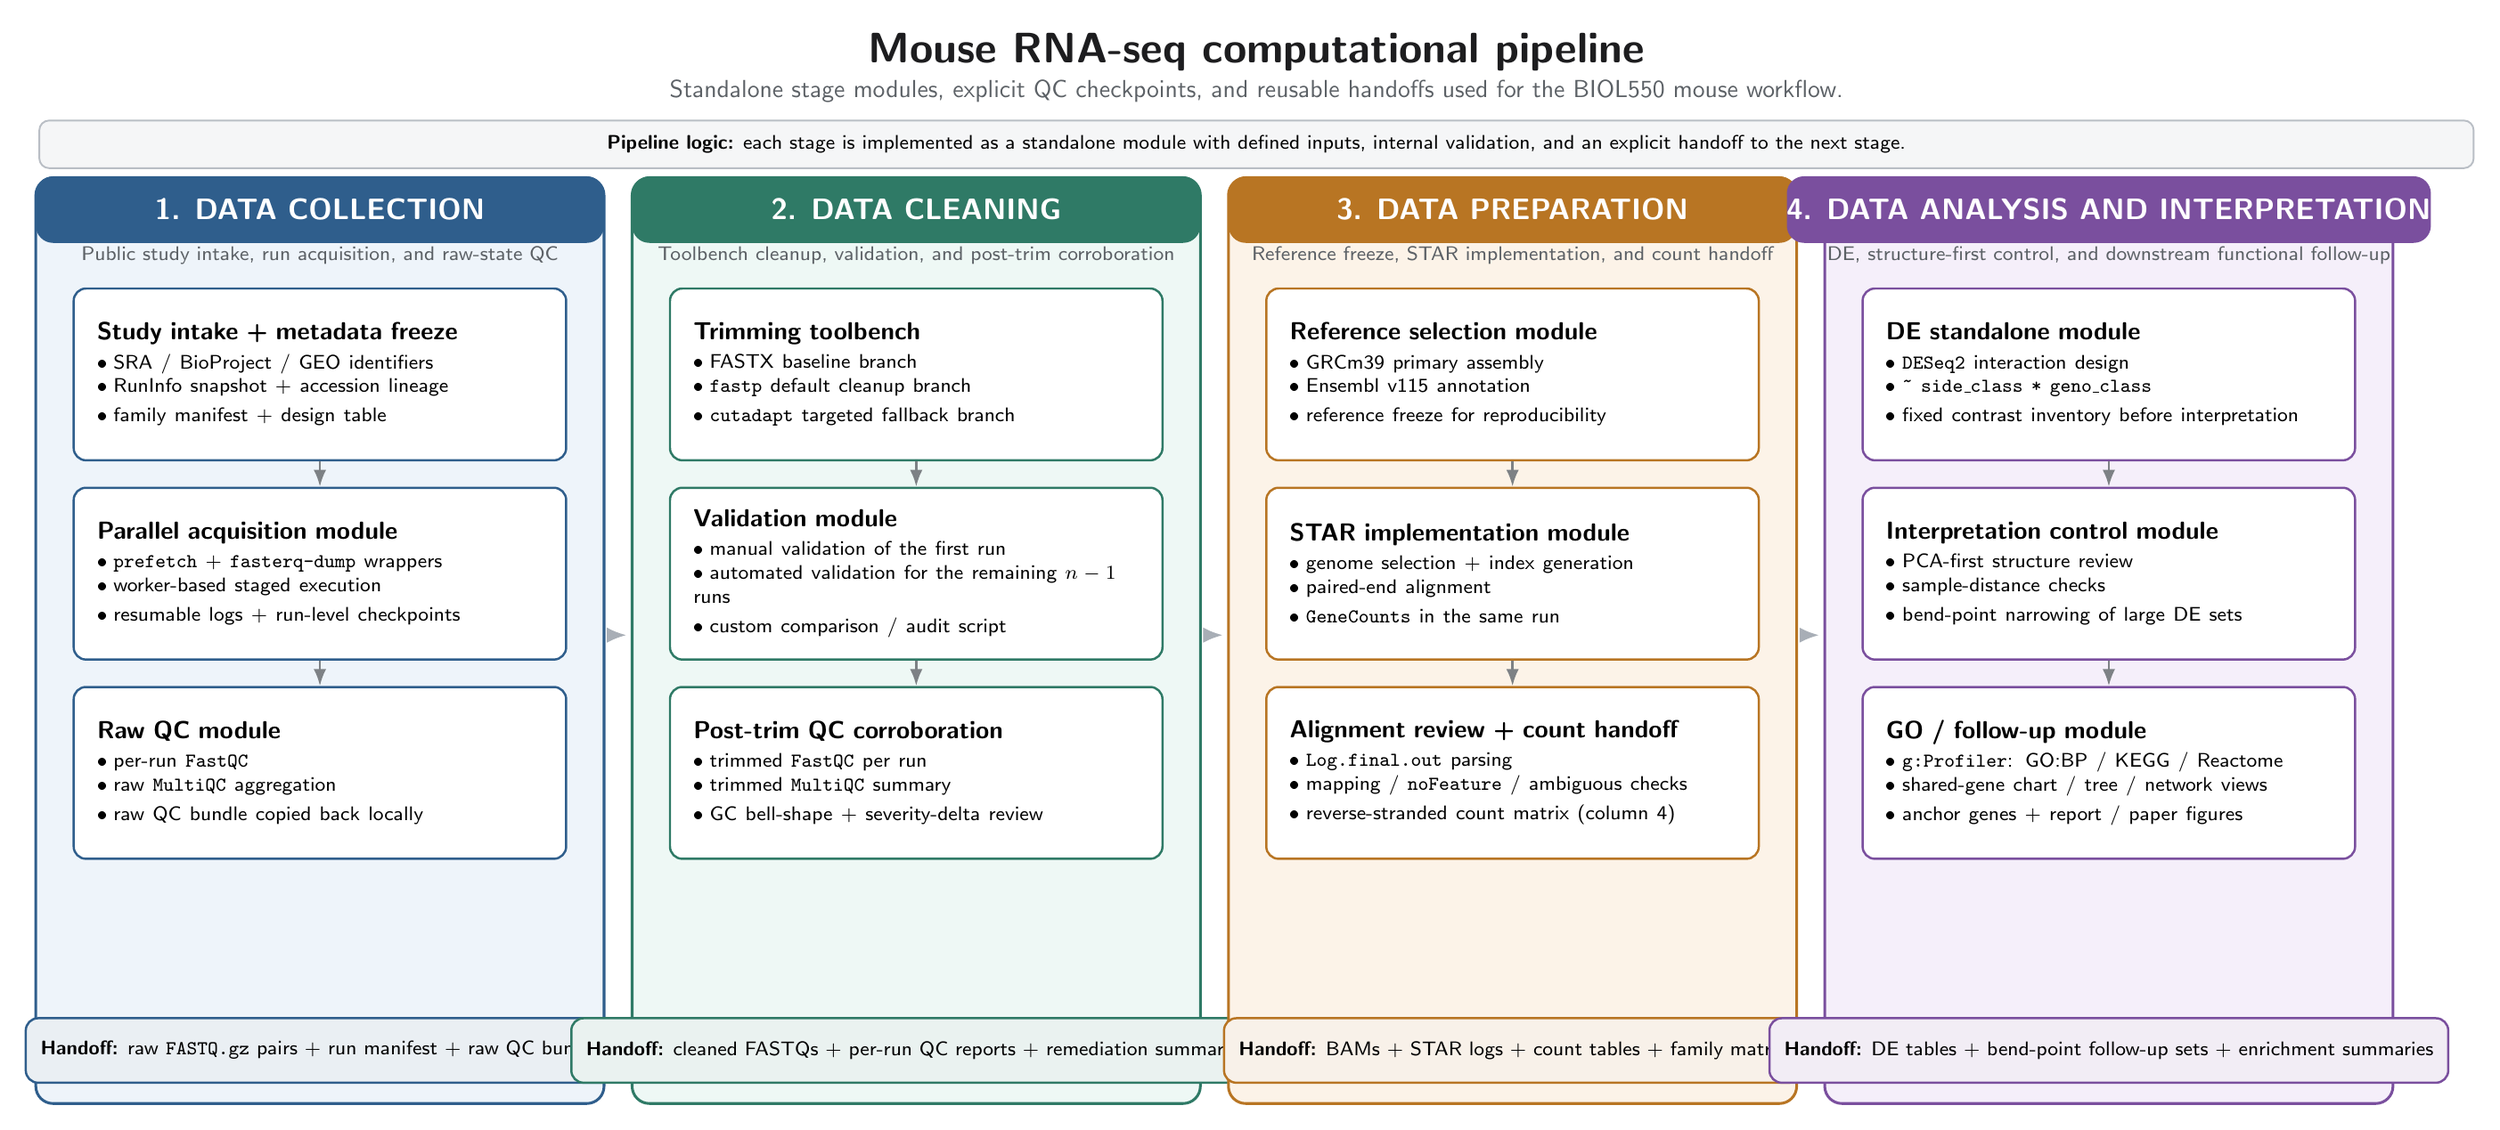
\begin{tikzpicture}[x=1cm,y=1cm]

\node[font=\bfseries\fontsize{18}{20}\selectfont, text=ink] at (17.9,14.85) {Mouse RNA-seq computational pipeline};
\node[font=\fontsize{9.8}{11}\selectfont, text=muted, align=center] at (17.9,14.28)
{Standalone stage modules, explicit QC checkpoints, and reusable handoffs used for the BIOL550 mouse workflow.};
\node[note, minimum width=34.7cm, minimum height=0.68cm, align=center] at (17.9,13.53)
{{\bfseries\fontsize{8.3}{9.2}\selectfont Pipeline logic:} each stage is implemented as a standalone module with defined inputs, internal validation, and an explicit handoff to the next stage.};

\def\stageTop{6.45}
\def\stageW{8.1}
\def\modW{7.02}
\def\modH{2.45}
\def\gap{0.36}

% Stage 1
\node[stage, draw=collect, fill=collectbg, minimum width=\stageW cm] (S1) at (4.55,\stageTop) {};
\node[stagehead, fill=collect, minimum width=\stageW cm] at ($(S1.north)+(0,-0.47)$) {1. DATA COLLECTION};
\node[font=\fontsize{8.25}{9.25}\selectfont, text=muted, align=center] at ($(S1.north)+(0,-1.12)$) {Public study intake, run acquisition, and raw-state QC};

\node[modulebox, draw=collect, minimum width=\modW cm, text width=6.35cm, minimum height=\modH cm, anchor=north] (c1) at ($(S1.north)+(0,-1.58)$) {\modtitle{Study intake + metadata freeze}\\[2pt]
\modbody{\bul SRA / BioProject / GEO identifiers\\
\bul RunInfo snapshot + accession lineage\\
\bul family manifest + design table}};

\node[modulebox, draw=collect, minimum width=\modW cm, text width=6.35cm, minimum height=\modH cm, anchor=north] (c2) at ($(c1.south)+(0,-\gap)$) {\modtitle{Parallel acquisition module}\\[2pt]
\modbody{\bul \texttt{prefetch} + \texttt{fasterq-dump} wrappers\\
\bul worker-based staged execution\\
\bul resumable logs + run-level checkpoints}};

\node[modulebox, draw=collect, minimum width=\modW cm, text width=6.35cm, minimum height=\modH cm, anchor=north] (c3) at ($(c2.south)+(0,-\gap)$) {\modtitle{Raw QC module}\\[2pt]
\modbody{\bul per-run \texttt{FastQC}\\
\bul raw \texttt{MultiQC} aggregation\\
\bul raw QC bundle copied back locally}};

\node[handoff, draw=collect, fill=collect!10, minimum width=7.22cm, minimum height=0.92cm, anchor=south] (h1) at ($(S1.south)+(0,0.30)$) {\textbf{Handoff:} raw \texttt{FASTQ.gz} pairs + run manifest + raw QC bundle};

% Stage 2
\node[stage, draw=clean, fill=cleanbg, minimum width=\stageW cm] (S2) at (13.05,\stageTop) {};
\node[stagehead, fill=clean, minimum width=\stageW cm] at ($(S2.north)+(0,-0.47)$) {2. DATA CLEANING};
\node[font=\fontsize{8.25}{9.25}\selectfont, text=muted, align=center] at ($(S2.north)+(0,-1.12)$) {Toolbench cleanup, validation, and post-trim corroboration};

\node[modulebox, draw=clean, minimum width=\modW cm, text width=6.35cm, minimum height=\modH cm, anchor=north] (d1) at ($(S2.north)+(0,-1.58)$) {\modtitle{Trimming toolbench}\\[2pt]
\modbody{\bul FASTX baseline branch\\
\bul \texttt{fastp} default cleanup branch\\
\bul \texttt{cutadapt} targeted fallback branch}};

\node[modulebox, draw=clean, minimum width=\modW cm, text width=6.35cm, minimum height=\modH cm, anchor=north] (d2) at ($(d1.south)+(0,-\gap)$) {\modtitle{Validation module}\\[2pt]
\modbody{\bul manual validation of the first run\\
\bul automated validation for the remaining \(n-1\) runs\\
\bul custom comparison / audit script}};

\node[modulebox, draw=clean, minimum width=\modW cm, text width=6.35cm, minimum height=\modH cm, anchor=north] (d3) at ($(d2.south)+(0,-\gap)$) {\modtitle{Post-trim QC corroboration}\\[2pt]
\modbody{\bul trimmed \texttt{FastQC} per run\\
\bul trimmed \texttt{MultiQC} summary\\
\bul GC bell-shape + severity-delta review}};

\node[handoff, draw=clean, fill=clean!10, minimum width=7.22cm, minimum height=0.92cm, anchor=south] (h2) at ($(S2.south)+(0,0.30)$) {\textbf{Handoff:} cleaned FASTQs + per-run QC reports + remediation summaries};

% Stage 3
\node[stage, draw=prep, fill=prepbg, minimum width=\stageW cm] (S3) at (21.55,\stageTop) {};
\node[stagehead, fill=prep, minimum width=\stageW cm] at ($(S3.north)+(0,-0.47)$) {3. DATA PREPARATION};
\node[font=\fontsize{8.25}{9.25}\selectfont, text=muted, align=center] at ($(S3.north)+(0,-1.12)$) {Reference freeze, STAR implementation, and count handoff};

\node[modulebox, draw=prep, minimum width=\modW cm, text width=6.35cm, minimum height=\modH cm, anchor=north] (p1) at ($(S3.north)+(0,-1.58)$) {\modtitle{Reference selection module}\\[2pt]
\modbody{\bul GRCm39 primary assembly\\
\bul Ensembl v115 annotation\\
\bul reference freeze for reproducibility}};

\node[modulebox, draw=prep, minimum width=\modW cm, text width=6.35cm, minimum height=\modH cm, anchor=north] (p2) at ($(p1.south)+(0,-\gap)$) {\modtitle{STAR implementation module}\\[2pt]
\modbody{\bul genome selection + index generation\\
\bul paired-end alignment\\
\bul \texttt{GeneCounts} in the same run}};

\node[modulebox, draw=prep, minimum width=\modW cm, text width=6.35cm, minimum height=\modH cm, anchor=north] (p3) at ($(p2.south)+(0,-\gap)$) {\modtitle{Alignment review + count handoff}\\[2pt]
\modbody{\bul \texttt{Log.final.out} parsing\\
\bul mapping / \texttt{noFeature} / ambiguous checks\\
\bul reverse-stranded count matrix (column 4)}};

\node[handoff, draw=prep, fill=prep!10, minimum width=7.22cm, minimum height=0.92cm, anchor=south] (h3) at ($(S3.south)+(0,0.30)$) {\textbf{Handoff:} BAMs + STAR logs + count tables + family matrix};

% Stage 4
\node[stage, draw=analysis, fill=analysisbg, minimum width=\stageW cm] (S4) at (30.05,\stageTop) {};
\node[stagehead, fill=analysis, minimum width=\stageW cm] at ($(S4.north)+(0,-0.47)$) {4. DATA ANALYSIS AND INTERPRETATION};
\node[font=\fontsize{8.25}{9.25}\selectfont, text=muted, align=center] at ($(S4.north)+(0,-1.12)$) {DE, structure-first control, and downstream functional follow-up};

\node[modulebox, draw=analysis, minimum width=\modW cm, text width=6.35cm, minimum height=\modH cm, anchor=north] (a1) at ($(S4.north)+(0,-1.58)$) {\modtitle{DE standalone module}\\[2pt]
\modbody{\bul \texttt{DESeq2} interaction design\\
\bul \texttt{\~{} side\_class * geno\_class}\\
\bul fixed contrast inventory before interpretation}};

\node[modulebox, draw=analysis, minimum width=\modW cm, text width=6.35cm, minimum height=\modH cm, anchor=north] (a2) at ($(a1.south)+(0,-\gap)$) {\modtitle{Interpretation control module}\\[2pt]
\modbody{\bul PCA-first structure review\\
\bul sample-distance checks\\
\bul bend-point narrowing of large DE sets}};

\node[modulebox, draw=analysis, minimum width=\modW cm, text width=6.35cm, minimum height=\modH cm, anchor=north] (a3) at ($(a2.south)+(0,-\gap)$) {\modtitle{GO / follow-up module}\\[2pt]
\modbody{\bul \texttt{g:Profiler}: GO:BP / KEGG / Reactome\\
\bul shared-gene chart / tree / network views\\
\bul anchor genes + report / paper figures}};

\node[handoff, draw=analysis, fill=analysis!10, minimum width=7.22cm, minimum height=0.92cm, anchor=south] (h4) at ($(S4.south)+(0,0.30)$) {\textbf{Handoff:} DE tables + bend-point follow-up sets + enrichment summaries};

% internal arrows
\draw[vflow] (c1.south) -- (c2.north);
\draw[vflow] (c2.south) -- (c3.north);
\draw[vflow] (d1.south) -- (d2.north);
\draw[vflow] (d2.south) -- (d3.north);
\draw[vflow] (p1.south) -- (p2.north);
\draw[vflow] (p2.south) -- (p3.north);
\draw[vflow] (a1.south) -- (a2.north);
\draw[vflow] (a2.south) -- (a3.north);

% stage-to-stage arrows
\draw[flow] ($(S1.east)+(0.06,0.08)$) -- ($(S2.west)+(-0.06,0.08)$);
\draw[flow] ($(S2.east)+(0.06,0.08)$) -- ($(S3.west)+(-0.06,0.08)$);
\draw[flow] ($(S3.east)+(0.06,0.08)$) -- ($(S4.west)+(-0.06,0.08)$);

\end{tikzpicture}
\end{document}
